

\section{Query Compilation}
\label{sec:compiler}


This section describes the Cumulus query compiler.

TODO: provide introduction and overview to the section. Fill in missing part
on how negated calculus is handled in delta processing. Provide
pseudocode for compilation algorithm. Explain how ``for x m[x] += if(x=b) ...''
is turned into ``x[b] += ...''. Compile running example.


\subsection{Cumulus Query Calculus and M3F}


\def\safe{\mbox{safe}}
\def\AggSum{\mbox{Sum}}

Our calculus consists of
{\em formulae} of positive quantifier-free relational domain calculus
(i.e., formulae constructed from conjunctions ``and'',
disjunctions ``or'', and atoms) and of {\em terms}.
%
The atomic formulae are {\em true}, {\em false}, relational atoms $R(\vec{x})$
where $\vec{x}$ is a tuple of variables,
and atomic constraints of the form $t_1 \;\theta\; t_2$ comparing two terms
$t_1$ and $t_2$ using comparison operations $\theta$ of $=$, $\neq$, $<$,
and $\leq$.
%
Terms are built from variables, constants, built-in function calls
$f(\vec{t})$, where $\vec{t}$ is a tuple of terms,
and aggregrate sums ($\AggSum$) using addition and multiplication.
Built-in functions compute their result entirely based on their input
terms, not accessing the database (e.g., mod or string concatenation).
In short, the grammar for formulae $\phi$ and terms $t$
(given variables $x$, constants $c$, relation names $R$,
comparison operators $\theta$,
and builtin functions $f$) is
\begin{eqnarray*}
  \phi &\mbox{::-}& \phi \land \phi
               \mid \phi \lor \phi \mid (\phi)
               \mid \mbox{true} \mid \mbox{false} \mid R([x(,x)^*])
               \mid t \;\theta\; t
\\
  t &\mbox{::-}& t * t \mid t + t \mid (t) \mid c \mid x \mid f([t(,t)^*]) \mid
                 \AggSum(t, \phi)
\end{eqnarray*}

An aggregate term $\AggSum(t, \phi)$
is {\em constraints-only} if $\phi$ does not
contain relational atoms $R(\vec{x})$ (but atomic constraints $s \theta t$).
Given just the bound variables, all variables
occurring in $\phi$ are safe and we can determine the truth value of
$\phi$. We can also think of such an aggregate term as a (functional)
if-statement (if $\phi$ then t else 0)
or, using C syntax, ($\phi$ ? $t$ : 0).

We will make one important syntactic restriction, namely that
no $\AggSum$ terms may occur in atomic constraints.

Formulas and terms are evaluated relative to a given set of
{\em bound variables}.
The bound variables of a subformula are the bound variables of the formula.

Given a set of bound variables $B$,
the {\em safe variables} of a formula are defined bottom-up
as usual in relational
calculus (see e.g. \cite{DBLP:books/aw/AbiteboulHV95}). In particular,
\begin{eqnarray*}
\safe_B(R(\vec{x})) &:=& \{x_i\} \cup B \\
\safe_B(\phi \land \psi) &:=& \safe_B(\phi) \cup \safe_B(\psi) \\
\safe_B(\phi \lor \psi)  &:=& \safe_B(\phi) \cap \safe_B(\psi) \\
\safe_B(\phi \land x = y) &:=&
\left\{\begin{array}{ll}
\safe_B(\phi) \cup \{ x, y \} &\dots
\mbox{$x$ or $y$ is} \\
&\;\;\; \mbox{in $\safe_B(\phi)$} \\[.5ex]
\safe_B(\phi) &\dots \mbox{otherwise}.
\end{array} \right.
\end{eqnarray*}
Here $\{x_i\}$ drops order and turns the tuple $\vec{x}$ into a set.

Given a term $\AggSum(t, \phi)$ with bound variables $B$,
the bound variables of $\phi$ are $B$ and the bound variables of $t$ are
the safe variables of $\phi$, $\safe_B(\phi)$.
The bound variables of a subterm are the bound variables of the term.
Variables occuring as terms must be bound.

\begin{example}\em
Given singleton bound variable set $\{ y \}$,
\[ \AggSum(u * f(z), \underbrace{(\underbrace{(\underbrace{R(x, z)}_{x,y,z} \lor \underbrace{y=z}_{y,z})}_{y,z} \land z = w)}_{y,z,w}) \]
is invalid: The safe variables of the formula are
$\{y,z,w\}$, so $u$ is not bound in the term $u * f(z)$. The overall term
becomes valid for bound variables $\{u,y\}$.
\punto
\end{example}


\def\db{{\cal{A}}}

The semantics of formulas and terms is given by a (polymorphic) function
$\Bracks{\cdot}(\cdot, \cdot)$ that takes a database and values for the
bound variables as arguments. Given database $\db$ and values $\vec{b}$ for
the bound variables,
$\Bracks{\phi}(\db, \vec{b})$ evaluates to a relation and
$\Bracks{t}(\db, \vec{b})$ evaluates to a value of the type of
terms.\footnote{In practice,
we have several types such as integers and floats, but
here we will not talk about types and will assume that all terms evaluate to,
say, floating point numbers. However, our implementation supports the
main data types of SQL, and no noteworthy observations were made achieving
this.}
We assume a multiset semantics for relations, which is important to note
since we focus on computing aggregates. The multiset semantics of formulas
is defined by their well-known translation to relational algebra
(Codd's theorem), and the standard multi-set semantics of
(in our case, positive) relational algebra. 
$\AggSum$ terms are new, but otherwise the
semantics of terms is obvious.
A term $\AggSum(t, \phi)$
computes the sum of the values $t[\vec{x}]$
over the distinct valuations (with duplicates)
of the safe variables $\vec{x}$ of $\phi$, i.e.,
given a database $\db$ and values $\vec{b}$ for the bound variables of $\phi$,
\[
\Bracks{\AggSum(t, \phi)}(\db, \vec{b}) =
\sum_{\vec{v} \;\mathrm{in}\; \Bracks{\phi}(\db, \vec{b})} \Bracks{t}(\db, \vec{v}).
\]


\subsection{From SQL to the Calculus}


Given our semantics definition, the translation from SQL to our calculus is
straightforward. We focus on aggregation queries, specifically
sum aggregation queries (count and avg aggregation queries can be encoded
using sum). Aggregates can be nested in the SELECT clause, but not in
the FROM, WHERE, or HAVING clause. We support GROUP by, although in a way
that may at first seem nonstandard. We do not support DISTINCT.
A SQL aggregate query
\begin{verbatim}
SELECT groupcols, SUM(t)
FROM   R1 r11, R1 r12, ..., R2 r21, ...
WHERE  cond
GROUP BY groupcols
\end{verbatim}
is encoded in the calculus as
\[
\AggSum(t, R_1(\vec{x}_{11}) \land R_1(\vec{x}_{12}) \land \dots
\land R_2(\vec{x}_{21}) \land \dots \land \mbox{cond})
\]
with {\em bound variables} groupcols.
For example,
\begin{verbatim}
SELECT R.A, SUM(R.B) FROM R GROUP BY R.A
\end{verbatim}
maps to
$\AggSum(y, R(x,y))$ with bound variable $x$ assuming that the schema of
$R$ is $(A,B)$.
We will see more interesting examples of this translation later.


\subsection{Normalization and Simplification}


A semiring is an algebra with two associative operations,
$+$ and $*$, that
have neutral elements (called 0 and 1, respectively), which satisfy
distributivity ($a*(b+c)= a*b + a*c$), and where $+$ is commutative.
Semirings with variables
have polynomials, that is, each expression of the
semiring can be mapped to an equivalent expression that is
a sum of flat products (the products are also known as {\em monomials}\/).
Turning semiring expressions into polynomials just means to apply
distributivity repeatedly until we end up with a polynomial.
This can be combined with simplification operations based on the 1 and
0-elements, i.e., $\alpha * 1$ maps to $\alpha$, $\alpha*0$ maps to $0$, and
$\alpha+0$ maps to $\alpha$. Polynomials can be conveniently implemented
as lists of lists of atoms, where an empty top-level list (i.e., polynomial)
has value 0 and an empty monomial list has value 1.

Both our formulae and our terms are semirings; in particular,
in the semiring of formulae, $\land$ is the product operation,
$\lor$ is addition,
and $\textit{false}$ and $\textit{true}$ are 0 and 1, respectively.

For arbitrary terms $s$ and $t$ and formulas $\phi$ and $\psi$,
$\AggSum$ terms can be simplified using the following equations (to be
applied by replacing a left by a right hand side expression)
\begin{eqnarray*}
\AggSum(t, \textit{true}) &=& t \\
\AggSum(t, \textit{false}) &=& 0 \\
\AggSum(0, \phi) &=& 0 \\
\AggSum(s+t, \phi) &=& \AggSum(s, \phi) + \AggSum(t, \phi) \\
\AggSum(t, \phi \lor \psi) &=& \AggSum(t, \phi) + \AggSum(t, \psi)
\end{eqnarray*}

All these algebraic laws can be applied, and the calculus expression
be maximally simplified, in a single bottom-up pass of the expression.
A term ($\AggSum$ or other) maximally simplified in this way
is a sum of terms that contain neither $+$ nor $\lor$; we call such 
normalized terms {\em recursively monomial}.

\def\vars{\mbox{vars}}

{\bf Factorization of monomial aggregate terms}.
For expression $e$ either a formula or a term, let $\vars(e)$
be the set of all variables occurring in $e$.
Factorization employs the equivalence
\[
\AggSum(s*t, \phi \land \psi) = \AggSum(s, \phi) * \AggSum(t, \psi)
\]
which is true if
$(\vars(s) \cup \vars(\phi)) \cap (\vars(t) \cup \vars(\psi)) = \emptyset$.

Consider an aggregate term $\AggSum(t, \phi)$ where both $t$ and $\phi$ are
monomials, consisting of the sets $T$ and $F$ of atomic terms and formulae,
respectively (that is, $t = \prod T$ and $\phi = \bigwedge F$).
We can think of the
elements of the two-sorted set $T \cup F$ as the hyperedges of a
{\em hypergraph},
where the function $\vars(e)$ maps hyperedge $e$ to the nodes that are
part of it.
The set of {\em connected components} ${\cal C}$ of this hypergraph is the
maximum cardinality set of subsets of $T \cup F$ such that for any
two components $C_1, C_2 \in {\cal C}$ with $C_1 \neq C_2$,
$\vars(C_1) \cap \vars(C_2) = \emptyset$. Asking for the maximum number of
nonoverlapping components is of course the same as asking for components of
minimum size, and the set of connected components is unique and can be computed
in linear time using Tarjan's algorithm. Given ${\cal C}$, each component
$C \in {\cal C}$ can again be partitioned by sort into a monomial term $t_C$
and a monomial formula $\phi_C$.
%
% By convention, if $C$ does not contain atomic terms, $t_C = 1$ and if $C$
% does not contain atomic formulae, $\phi_C = \textit{true}$. It is not
% difficult to verify that
%
$\AggSum(t, \phi)$ is equivalent to
\[
\prod_{C \in {\cal C}} \AggSum(t_C, \phi_C).
\]

\begin{example}\em
The connected components of term
\[
\AggSum(5 * x * \AggSum(1, R(y, z)) * w, R(x,y) \land S(z) \land R(v, w))
\]
are
$\{ \{5\}, \{ x, R(x,y), \AggSum(1, R(y, z)), S(z) \}$,
$\{ w, R(v, w)) \} \}$
and thus the term factorizes as
$\AggSum(5, \textit{true}) *
\AggSum(x * \AggSum(1$, $R(y, z)), R(x, y) \land S(z)) *
\AggSum(w, R(v, w)))$.
$\AggSum(5, \textit{true})$ simplifies to $5$.
\punto
\end{example}


{\bf Variable elimination}.
Given an abitrary monomial formula $\phi = \bigwedge (E, O)$,
where $E$ are the equality
atoms $x=y$ and $O$ are the remaining atoms (either set may be empty) and
a set of bound variables $B$.
We eliminate redundant variables as follows.

Consider the equivalence classes of the equivalence relation $E$.
For each equivalence class $C$ of $E$, distinguish an element
(i.e., variable) as $x_C$ such that,
if $B \cap C \neq \emptyset$, $x_C$ is an arbitrary element of $B \cap C$;
otherwise, it is an arbitrary element of $C$.
Create a unification mapping
$\Theta$ that maps each unbound variable $y$ of $E$ to $x_{[y]}$ (where $[y]$ is the
equivalence class of $y$) and is the identity on the bound variables.
Now substitute all variables in $O$
using $\Theta$, obtaining $O'$. Let
$E' =  \bigcup \{ y = x_{[y]} | y \in ((B \cap [y]) -  x_{[y]}) \}$.
Then we replace $\phi$ by $(\bigwedge O') \land \bigwedge E'$.

Given a term $\AggSum(t,\phi)$ where $\phi$ is a monomial,
and bound variables, we eliminate variables by 
first eliminating variables in $\phi$, creating $\phi'$ and $\Theta$.
Then we substitute all variables of $t$ that are in the domain of $\Theta$
using $\Theta$, obtaining $t'$. The result, $\AggSum(t', \phi')$, is equivalent
to $\AggSum(t,\phi)$.


\begin{example} \em
Given term $\AggSum(y*v*r, R(z, v) \land v<q
\land x=y \land x=z \land u=v \land v=w \land q=r)$
and bound variables $\{x,y,z,r\}$.
The variable equivalence classes are
$\{ \{x,y,z\}, \{u,v,w\}, \{q,r\} \}$. We chose the rightmost variable in
each class as the variable to substitute by. In the first class, we can choose
freely because all members are bound. In the second we can choose freely
because none are bound. In the third, we must choose $r$ because it is bound
and $q$ is not.
The mapping is
$\Theta = \{ x \mapsto x, y \mapsto y, z \mapsto z, u \mapsto w, v \mapsto w,
w \mapsto w, q \mapsto r, r \mapsto r \}$.
We apply $\Theta$ to $y*v*r$ and $R(z, v) \land v < q$ and obtain
$z*w*r$ and $R(z,w) \land w<r$, respectively. The simplified
overall term is
$\AggSum(z*w*r, R(z,w) \land w<r \land x=z \land y=z)$.
\punto
\end{example}


{\bf Extraction of aggregates}.
For a term $t$ and its set $B$ of bound variables,
the function ExtractAggregates($t$, $B$)
replaces each maximal subterm $s$ of $t$
that is of the form $\AggSum(\cdot, \cdot)$ but is not constraints-only
by a ``map access''  $m[\vec{x}]$, where
$m$ is a new name and $\vec{x}$ is the set of variables
both bound at $s$ and used in $s$ ordered arbitrarily.
The result of ExtractAggregates thus is a pair $(t', \Theta)$ of the remainder
term $t'$ and a mapping $\Theta$ from map accesses $m[\vec{x}]$ to extracted
subterms $s$ (which could be used to undo the extraction).

\begin{example}\em
Let $t$ be the term
\begin{multline*}
\AggSum(x*\AggSum(w, R(v, w), R(w, z)), x<y \land y=z) \\
*\; 5 * y * \AggSum(u, R(u, x)).
\end{multline*}
Then ExtractAggregates($t$, $\{x,y\}$) returns the pair consisting of term
$\AggSum(x*m_1[z], x<y \land y=z) * 5 * y * m_2[x]$
and the mapping
$\{
m_1[z] \mapsto \AggSum(w, R(v, w), R(w, z));
m_2[x] \mapsto \AggSum(u, R(u, x))
\}$.
\punto
\end{example}


\subsection{Delta Computation}


\def\dt{\Delta_{\pm R(\vec{t})}}


Given a term or formula $\alpha$
of our calculus, and an insertion or deletion of a
single tuple $\vec{t}$ to/from a relation $R$ of the database.
We denote the database obtained from database $\db$ by this update by
$\db \pm R(\vec{t})$.
We can express a delta $\Delta_{\pm R(\vec{t})} \alpha$
(which is a term if $\alpha$ is a term and a formula if $\alpha$ is a formula)
such that,
given current database $\db$ and values $\vec{b}$ for the bound variables,
\begin{eqnarray}
\Bracks{\alpha}(\db \pm R(\vec{t}), \vec{b}) &=&
\,\Bracks{\alpha}(\db) \pm \,\Bracks{\dt \alpha}(\db, \vec{b})
\label{eq:delta}
\end{eqnarray}
as follows.

The delta rules for semirings are as follows. We use $+$ and $*$ for the
addition and multiplication operations; for formulae, these are of course
$\lor$ and $\land$, respectively.
\[\begin{array}{lllcr}
\dt (\alpha + \beta) &:=& ((\dt \alpha)    &+& (\dt \beta))
\\[1ex]
\dt (\alpha \,*\, \beta)
   &:=& ((\dt \alpha)               &*& \beta\;\,) \\
   &+ & (\quad\quad\quad\;\, \alpha &*& (\dt \beta)) \\
   &+ & ((\dt \alpha)               &*& (\dt \beta))
\end{array}\]

For atomic formulae and terms,
\[\begin{array}{lllr}
\dt \AggSum(t, \phi)
   &:=& \AggSum((\dt t), & \phi\;\,) \\
   &+ & \AggSum(\quad\quad\quad\; \,t,  & (\dt \phi)) \\
   &+ & \AggSum((\dt t), & (\dt \phi))
\\[1ex]
\dt R(x_1, \dots, x_k) &:=& \pm \bigwedge_{i=1}^k (x_i = t_i)
\end{array}\]
and, for $S$ a relation different from $R$,
\[
\dt S(x_1, \dots, x_l) := \textit{false}.
\]
For all other atomic terms and formulae, $\dt$ is the zero-element
of their respective semirings (that is, $0$ and $\textit{false}$,
respectively.)


\begin{proposition}
This definition of $\dt$ satisfies Equation \ref{eq:delta}.
\end{proposition}

\begin{proof}
It is easy to see that our definition is correct in the case of insertions.
For the deletion case, all we need to show is that
\begin{equation}
\Delta_{-R(\vec{t})}(\alpha + \Delta_{+R(\vec{t})} \alpha) = \alpha.
\label{eq:delta2}
\end{equation}


\def\dtp{\Delta_{+}}
\def\dtm{\Delta_{-}}


We use $\dtp$ and $\dtm$ as shortcuts for $\Delta_{+R(\vec{t})}$
and $\Delta_{-R(\vec{t})}$, respectively.
Let $\alpha' = \alpha+\dtp\alpha$ and $\beta' = \beta+\dtp\beta$.
Consider the expression
\[
\overbrace{\color{white}{\alpha\beta +
\color{black}{\overbrace{\color{white}{
(\dtp \alpha)\beta + (\dtp \alpha)(\dtp \beta)
+ \alpha(\dtp \beta)}}^{\dtp (\alpha\beta)}}}}^{\alpha' \beta'}
\color{white}{+ (\dtp \alpha)(\dtp \beta)}
\]

\vspace{-14mm}

\[
\alpha\beta +
\underbrace{(\dtp \alpha)\beta + (\dtp \alpha)(\dtp \beta)}_{
(\dtp \alpha)\beta'}
+ \underbrace{
\alpha(\dtp \beta) + (\dtp \alpha)(\dtp \beta)}_{\alpha'(\dtp \beta)}
\]
Since $\alpha'\beta' = \alpha\beta + \dtp(\alpha\beta)$,
\begin{equation}
\dtp(\alpha\beta) + (\dtp\alpha)(\dtp\beta) =
(\dtp \alpha)\beta' + \alpha'(\dtp \beta).
\label{eq:delta3}
\end{equation}
We can verify by inspection of our definition that
\begin{equation}
\dtm(\alpha'\beta') + (\dtp \alpha)\beta' + \alpha'(\dtp \beta) =
(\dtp\alpha)(\dtp\beta).
\label{eq:delta4}
\end{equation}
Summing up Equations \ref{eq:delta3} and \ref{eq:delta4}, we obtain
\[
\dtp(\alpha\beta) + \dtm(\alpha'\beta') = 0,
\]
which proves Equation~\ref{eq:delta2}.
%\punto
\end{proof}


\def\duv{\Delta_{\pm R(u,v)}}

\begin{example}\em
Consider the query
\begin{verbatim}
SELECT SUM(r1.A * r2.B) FROM R r1, R r2
WHERE r1.B=r2.A;
\end{verbatim}
over relation $R$ of schema $(A,B)$
whose deltas on insertion/deletion of
$R$-tuples is
$\duv \AggSum(x*z, R(x,y) \land R(y,z))$ =
$\AggSum(x*z, \duv (R(x,y) \land R(y,z)))$
because $\duv (x*z) = 0$. Since
$\duv R(x,y) = (x=u \land y=v)$ and
$\duv R(y,z) = (y=u \land z=v)$,%
%
\begin{multline*}
\AggSum(x*z, \duv (R(x,y) \land R(y,z))) = \\
\AggSum(x*z, ((x=u \land y=v)^\pm \land R(y,z)) \\
\lor\;
 (R(x,y) \land (y=u \land z=v)^\pm) \\
\lor\;
 ((x=u \land y=v)^\pm \land (y=u \land z=v)^\pm)) =
\end{multline*}

\vspace{-6mm}

\begin{eqnarray*}
&\pm& \AggSum(x*z, x=u \land y=v \land R(y,z)) \\
&\pm& \AggSum(x*z, R(x,y) \land y=u \land z=v) \\
&+  & \AggSum(x*z, x=u \land y=v \land y=u \land z=v).
\end{eqnarray*}
Assuming no other bound variables than $u$ and $v$,
this simplifies to
$\pm \AggSum(u*z, R(v,z))
 \pm \AggSum(x*v, (R(x,u))
 +   (\mbox{if }(u=v) \mbox{ then }(u*v)\mbox{ else }0)$.

Now suppose $R$ currently stores $\{\!| (1,1), (1,1) |\!\}$
(i.e., two copies of tuple $(1,1)$; the query has value 4)
and we insert another copy of tuple $(1,1)$.
Then $\Delta_{+R(1,1)} = 2 + 2 + 1 = 5$, which is
correct: the new value of the query is 9. Now if we delete one of the tuples
$(1,1)$,
$\Delta_{-R(1,1)} = -3 -3 +1 = -5$, and we get back to query value 4. 
\punto
\end{example}


\nop{
Note that $u$ and $v$ are bound variables (to be treated like constants).
Thus, for instance,
$\AggSum(u, R(v, v))$ corresponds to SQL
select u from R where R.A=v and R.B=v,
where we assume that the schema of $R$ is $(A,B)$.
} % end nop


\subsection{Compilation Algorithm}
\label{sec:compilation-alg}


The compilation algorithm employs {\em recursive incremental view
maintenance}. The algorithm Compile($t$, $\vec{b}$) takes a term $t$ to be
compiled and a tuple of bound variables.
For each trigger to be created (that is, for schema $R_1, \dots, R_k$,
the triggers are $+R_1, -R_1, \dots, +R_k, -R_k$),
we apply $\Delta$ for that trigger to $t$ and then normalize and
apply variable simplification. This creates a list of recursively monomials.
In each term $t'$ of this list, we extract the non-constraints-only aggregate
subterms using ExtractAggregates. We union together the mappings of
extractions, and eliminate duplicates. These are the todos.
The remainder term does not contain aggregates, just variables, constants, *,
if-then-else constructs, and map lookups.
By this extraction, we are committing ourselves to incrementally maintaining
the map $m[\vec{x}] = s$. 
The remainder term is the trigger code. For each pair $(m[\vec{x}], s)$
of the todos, we recursively call Compile($s$, $\vec{x}$) to create the update
triggers for map $m$.

\begin{example}\em
Consider a simplified TPC-H like schema with relations O(K, R)
and L(K, P). Orders O have an order key K and the currence exchange rate R fixed for this order (for
foreign customers). Line items L have an {\em order} key
K and a price P. We compile the query
\begin{verbatim}
SELECT SUM(L.P * O.R) FROM O, L WHERE O.K = L.K
\end{verbatim}
which asks for the sum total of all LineItem prices weighted by the exchange
rates of their orders.

The corresponding calculus term is
\[
q[] = \AggSum(p*r, O(k, r) \land L(k, p)).
\]
There are no group-by columns, so we compile as Compile($q$, $\emptyset$, $t$).
We first compute the (insertion) delta for $O$,
\[
\Delta_{+O(k_{O}, r_{O})} q =
\AggSum(p*r, k=k_{O} \land r=r_{O} \land L(k, p))
\]
and simplify with bound variables $\{k_{O}, r_{O}\}$ to
\[
\AggSum(p, L(k_{O}, p))*r_{O}
\]
We extract aggregates to get the pair
\[
\big( m_O[k_{O}]*r_{O},
\{ m_O[k_{O}] \mapsto \AggSum(p, L(k_{O}, p)) \} \big)
\]
Thus $\Delta_{+O(k_{O}, r_{O})} q = m_O[k_{O}]*r_{O}$
and we have to incrementally maintain $m_O[k_O]$.
\begin{eqnarray*}
\Delta_{+L(k_{L}, p_{L})} q &=&
   \AggSum(p*r, O(k, r) \land k=k_{L} \land p=_{L}) \\
&=& p_{L} * m_L[k_{L}]
\end{eqnarray*}
with $m_L[k_{L}] = \AggSum(r, O(k_{L}, r))$ to be incrementally maintained.
We run Compile($m_O$, $\{k_{O}\}$, $\AggSum(p, L(k_{O}, p))$)
and Compile($m_L$, $\{k_{L}\}$, $\AggSum(r, O(k_{L}, r))$) and obtain
\begin{eqnarray*}
\Delta_{+O(k_{OO}, r_{OO})} m_O[k_O] &=& 0 \\
\Delta_{+L(k_{OL}, p_{OL})} m_O[k_O] &=& (k_{OL} = k_O) \;?\; p_{OL} \;:\; 0 \\
\Delta_{+O(k_{LO}, r_{LO})} m_L[k_L] &=& (k_{LO} = k_L) \;?\; r_{LO} \;:\; 0 \\
\Delta_{+L(k_{LL}, p_{LL})} m_L[k_L] &=& 0.
\end{eqnarray*}

We have to incrementally maintain the maps $m_O[\cdot]$ and
$m_L[\cdot]$ for all values in the domain of order keys (i.e., all the order
keys present in the database). However, for bound variables
$k_{OL}, p_{OL}$,
\[
\mbox{for each $k_O$ do $m_O[k_O]$ += $(k_{OL} = k_O) \;?\; p_{OL} \;:\; 0$}
\]
simplifies to $m_O[k_{OL}]$ += $p_{OL}$,
and an analogous simplification applies to $m_L[k_L]$ on insert into $O$.

Overall, we obtain the insertion triggers
\begin{verbatim}
on insert into O(kO,  rO ) { q[] += mO[kO]*rO }
on insert into L(kL,  pL ) { q[] += pL*mL[kL] }
on insert into L(kOL, pOL) { mO[kOL] += pOL }
on insert into O(kLO, rLO) { mL[kLO] += rLO }
\end{verbatim}
The deletion triggers are like the insertion triggers with += replaced by -=.
\punto
\end{example}


\begin{remark}[Implementation Advice]
\em
There have been, in total, five prototypes of our compiler, and
in each subsequent generation, our picture of the problem has become clearer.
The compiler precisely as described in the section has been implemented
in OCAML in less than 1500 lines of code. We caution the reader against
abandoning our choice of using a calculus perspective
in favor of relational algebra with aggregates, or of misunderstanding
the exact role of safe and bound variables as used in this section.
We have made these mistakes in the past, resulting in 
a very difficult, and by about an order of magnitude larger, piece of code.
It may not be easy to see, but we strongly believe that
our choices here are not theoretical pedantism,
but key to allowing for exact yet concise presentation
and painless implementation.
\end{remark}


\subsection{Keys and Foreign Key Constraints}


\begin{example}\em
Consider again the query of Example~\ref{ex:TPCH-Q12},
\begin{verbatim}
SELECT   C.cid, SUM(1)
FROM     Customer C, Order O, LineItem L
WHERE    C.cid=O.cid AND O.oid=L.oid
GROUP BY C.cid;
\end{verbatim}

The compilation algorithm of Section~\ref{sec:compilation-alg} yields the
following M3F program:
\begin{verbatim}
+Customer(cid, nation):
  q[cid] += qC[cid];
  foreach oid do qL[cid, oid] += qLC[oid, cid];
  qO1[cid] += 1

+Order(oid, cid, ...):
  q[cid] += qO1[cid]*qO2[oid];
  qC[cid] += qO2[oid];
  qL[cid, oid] += qO1[cid];
  qLC[oid, cid] += 1

+LineItem(oid, ...):
  foreach cid do  q[cid] += qL[cid, oid];
  foreach cid do qC[cid] += qLC[oid, cid];
  qO2[oid] += 1

+Customer(cid, nation):
  qO1[cid] += 1

+Order(oid, cid, ...):
  qL[cid, oid] += qO1[cid];

+LineItem(oid, ...):
  foreach cid do  q[cid] += qL[cid, oid];
\end{verbatim}
\end{example}


\begin{figure}
\begin{center}
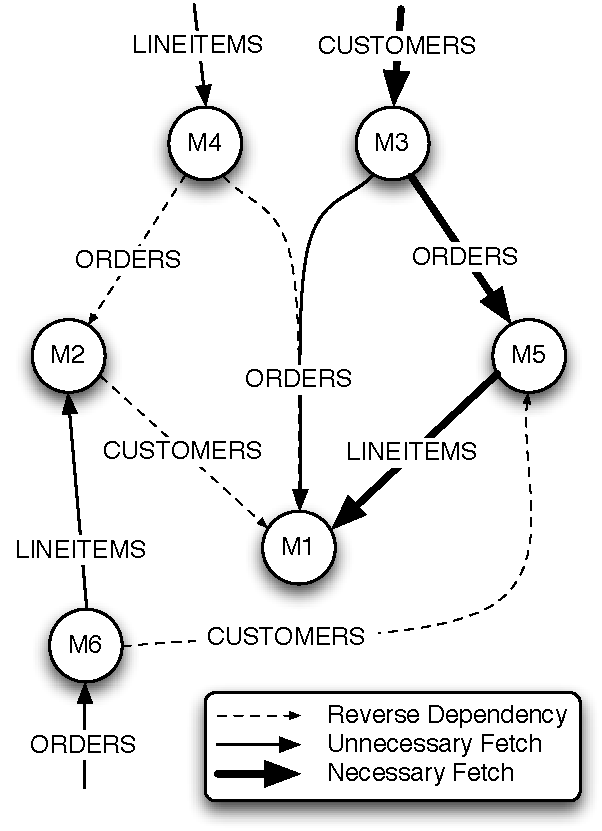
\includegraphics[width=2.5in]{images/q12_graph.pdf}
\caption{Data-flow graph for the example query.  Light and dashed edges can be optimized out, given foreign key constraints.
TODO: CHANGE MAP NAMES TO BE CONSISTENT WITH EXAMPLE; ROTATE FIGURE.}
\label{fig:dataflow}
\end{center}
\end{figure}



